% Activate the following line by filling in the right side. If for example the name of the root file is Main.tex, write
% "...root = Main.tex" if the chapter file is in the same directory, and "...root = ../Main.tex" if the chapter is in a subdirectory.
 
%!TEX root =  

\chapter{Methods}
\label{chapter4}
\section{Main ROS Principles}
\subsection{Inverse Kinematics}
dsaokdaskdaskldaskl;dsad
s
d;asdaskldksal;das
dsadsamdaskdkadklas;dsa\newline
lkjsakdsadjksajkdasjldas
\subsection{Visualisation using RViz}
dsaokdaskdaskldaskl;dsad
s
d;asdaskldksal;das
dsadsamdaskdkadklas;dsa\newline
lkjsakdsadjksajkdasjldas
\subsection{Fixed Frame Transforms}
A key aspect of creating the integrated movement system was understanding the concept of fixed frames and transforms. In ROS, Baxter contains information for multiple transforms between every joint and sections of his body. These transforms are known at all times to help know where a point is relative to one part, say the hand, against Baxter's torso. This method works similarly for the Kinect, where Baxter's torso coordinate system, is linked to the Kinect's coordinate system via a transform, which can be accessed by certain methods in ROS.

\begin{minipage}{0.65\textwidth}
\bigskip
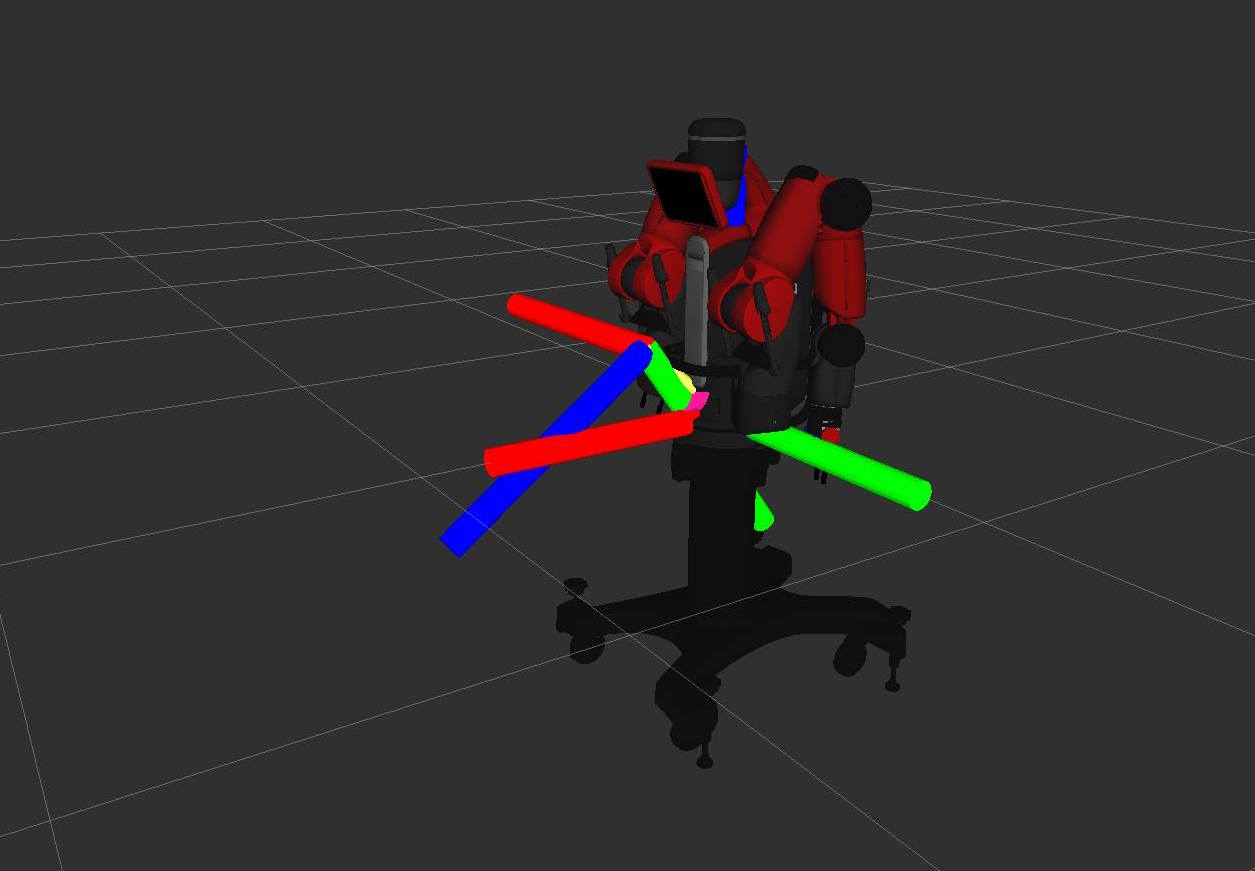
\includegraphics[width = 10cm, height = 6.5cm]{fixedframe.jpg}
\captionof{figure}{\textit{Example RVIZ Image}}
\bigskip
\end{minipage}
\hspace{0.5cm}
\begin{minipage}{0.29\textwidth}
\raggedright
Fixed coordinate systems were constantly used in testing the vision systems in this project, mainly within rViz. Everytime a coordinate or shape was recognised within the vision system, they could be published to rViz using a PointStamped object, which can be published in a particular coordinate
\end{minipage}

 system. Therefore publishing in one frame, transforming then publishing it another, rViz can show whether a point is correctly detected and whether it is in the correct frame.
\newline
This principle was used in the bowl recognition system, where after the centre of the bowl was obtained, Baxter needed to know where the centre of the bowl was in it's main body coordinate system before a movement command could be made. The system then looked up the transform between the Kinect and Baxter's torso to transform the 3D coordinate between coordinate systems.
\subsection{Custom Service Requests}
The idea that Baxter's movements would all be based on the current states of his vision system - depending upon where both the sweets and the bowl were, there needed to be a method developed for Baxter's movement system to be able to request information from the vision system. This was implemented via Services, which is a method in ROS that allows a custom message to be sent, and then received between two nodes.

\section{The Vision System}
\subsection{Calibration and Setup}
\subsection{Basic Vision Techniques}
Throughout this section, there is going to be information on the complex vision techniques used to help Baxter identify the position of the bowl and the sweets on the table. Firstly, here is some background information on the simpler, smaller algorithms used with these:
\begin{itemize}
\item{\textbf{RANSAC} - dsjadsjda}
\item{\textbf{Contours} - dsjadsjda}
\item{\textbf{Gaussian Blurring} - dsjadsjda}
\end{itemize}

\subsection{Bowl Recognition}
\textbf{Pointcloud Segmentation and Recognition}
\newline
The Kinect produces a pointcloud, a set of 3D points in the Kinect's coordinates system. To recognise the bowl of sweets on the table, the vision sytem first separates objects from the points representing the table, then separates those points into individiual object clusters. To eliminate noise and find the bowl cluster, a colour segmentation is performed to find only the white objects on the table. After that, the bowl can then be found by looking for the rim of the bowl as a circle in 3D space. This process is carried out by multiple algorithms, as discussed here:
\newline
\newline
\textbf{1. Tabletop Object Detection/Segmentation} 
\newline
This method works by detecting the main table plane in the Pointcloud by detecting the dominant plane using RANSAC. Points above this plane are then considered to be objects on top of the table, which are then segmented from the points within the table plane. This results in a pointcloud devoid of any points belonging to the table.
\newline
\newline
\textbf{2. Region Growing Segmentation}
\newline
The purpose of this algorithm is to separate the points in the pointcloud into clusters, ones which are close enough to separate into individual objects on the table. The theory behind this algorithm is it takes in the indices and estimated normals of the Pointcloud and for each possible region, calculates a K-nearest neighbour search over the indices. 
\begin{minipage}[t]{0.30\textwidth}
\raggedright
During this search, it compares each point with another, checking first for a specified smoothness constraint, checking if the deviation between normals is within a specified angle. If that is satisfied, then the difference in curvature is tested, allocating the points to the appropriately separated clusters.
\end{minipage}
\hspace{0.5cm}
\begin{minipage}[t]{0.64\textwidth}
\smallskip
\centering
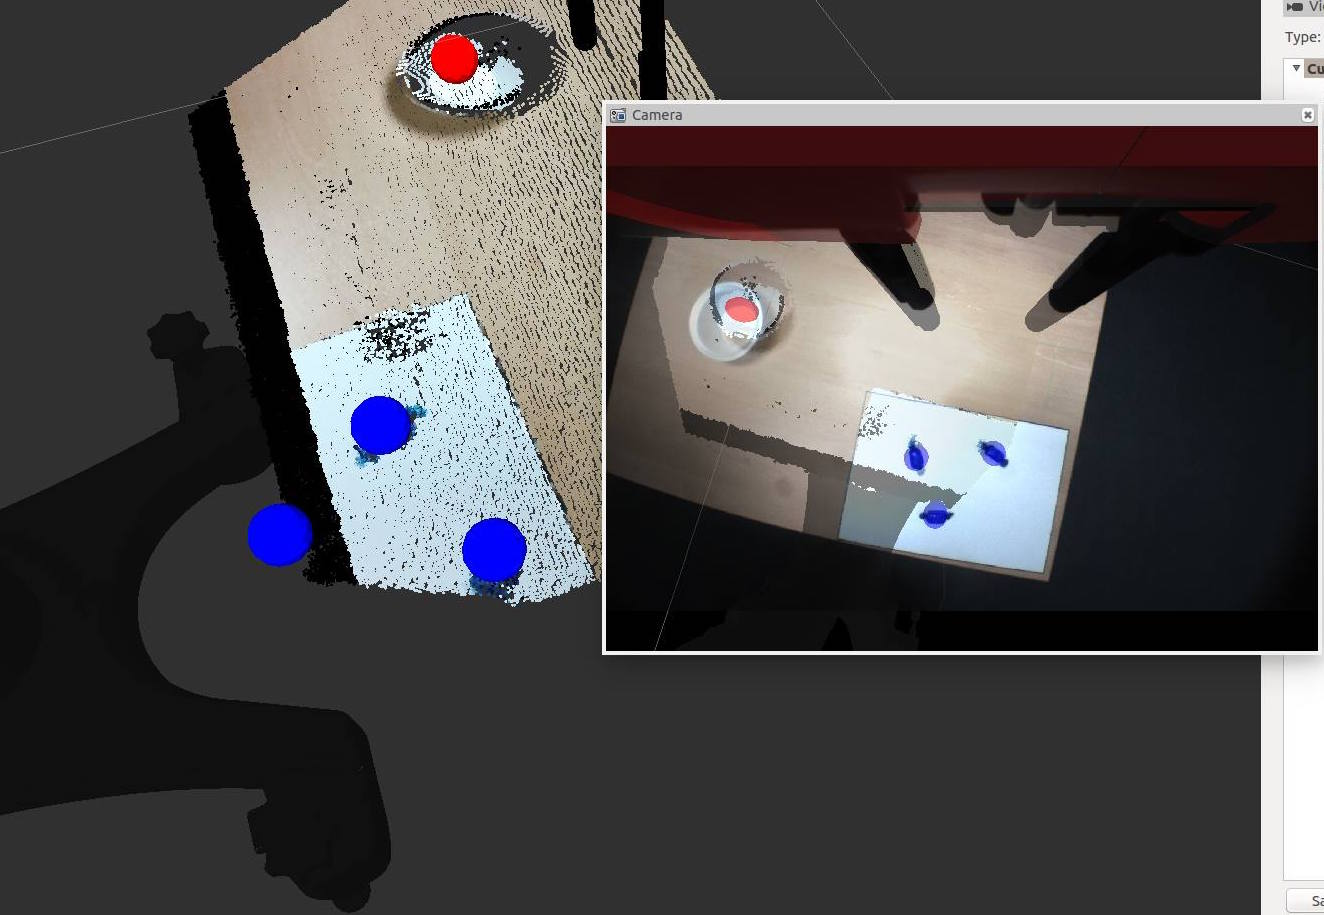
\includegraphics[width = 10cm, height = 6.5cm]{sweettransformation.jpg}
\centering
\captionof{figure}{\textit{An example of segmented objects}}
\bigskip
\bigskip
\end{minipage}
During the implementation of this algorithm, multiple number of neighbours, smoothness and curvature constraints were used until the individual objects in the pointcloud were sufficiently separated.
\newline
\newline
\textbf{3. Colour-Based Segmentation}
\newline
After separation of the Pointcloud into object clusters, a key thing to do was to get rid of noise caused by movement of Baxter's arms in front of the Kinect. 
\begin{minipage}[t]{0.64\textwidth}
\smallskip
\centering
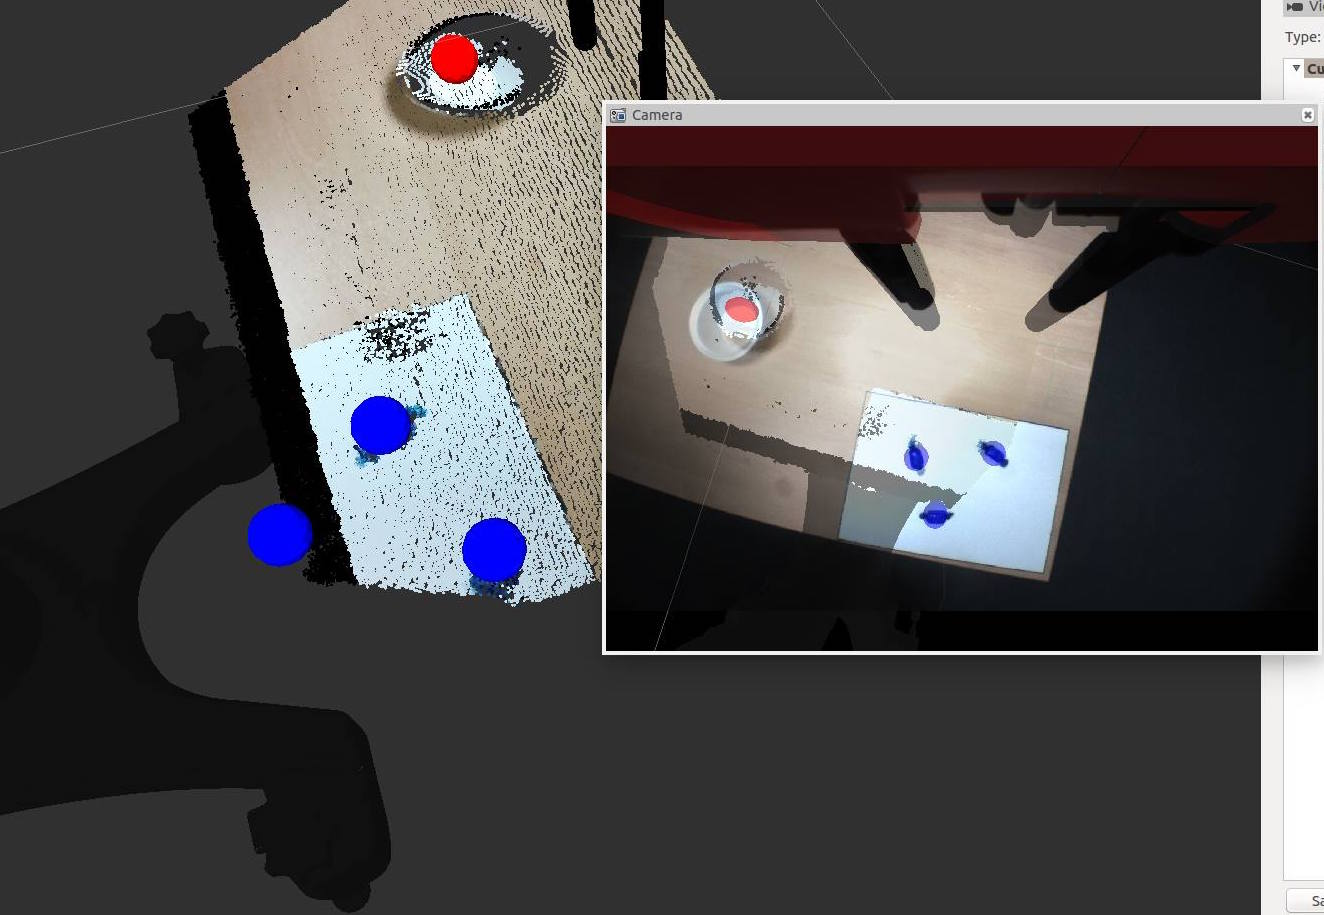
\includegraphics[width = 10cm, height = 6.5cm]{sweettransformation.jpg}
\centering
\captionof{figure}{\textit{An example of white colour segmented objects}}
\bigskip
\end{minipage}
\hspace{0.5cm}
\begin{minipage}[t]{0.29\textwidth}
\raggedright
To do this, black noise/points were eliminated by segmenting the objects further by colour. This was done by looping over the points in each cluster and averaging the RGB values of each cluster. Then, only the white clusters (those with a high enough R, G and B threshold), were
\end{minipage}	
segmented out so that the Pointcloud contains only the points for the bowl and any other white object on the table. This method could be expanded to recognise other colour bowl relatively easily, by finding the correct thresholds for other colour bowls.
\newline
\newline
\textbf{4. Detection of the Bowl Rim}
\newline
The most significant part of the bowl that tended to show up in the PointCloud was the bowl's rim. From that information, it was decided that the simplest solution was to find the rim of the bowl by finding a specific sized circle within a plane of the 3D PointCloud. This method was implemented by using the RANSAC algorithm to detect the points that best fit a circle shape within any plane. This method in the PCL library is especially good at allowing variation in it's detection. By varying distance thresholds and minimum/maximum circle radius values, the bowl was able to be found successfully, even with gaps in the rim, which occurred when Baxter's hands went in front of the bowl. After the circle model had been found in the white PointCloud, the x, y z of the centre of the bowl's rim was then known in the Kinect's frame coordinates.
\newline
\newline
\textbf{5. Improvement on Detection}
\newline
Due to the noise in the Kinect's Pointcloud recordings, some improvements were made further into development. The problem with the circle detection was that noise caused the centre of the bowl to shift each frame. To counteract the noise in detection, a cumulative average was taken over 20 frames and outputted as an average bowl centre. Then a cumulative centre point was taken further over time to de-noise the results, resulting in a fixed bowl centre that Baxter could reliably use as the actual centre of the bowl on the table.
\subsection{Sweet Recognition}
The task of Baxter recognising the sweets involved him being able to look at an area of the table with sweets retrieved from the bowl and determine how many sweets there were in that area along with what type/colour each sweet was. The problem with recognising the sweets using the Kinect is that the sweets were such small objects, that the noise in the Kinect meant that a significant number of sweets weren't picked up after segmenting objects on the table. Therefore an alternative method was proposed using OpenCV. The idea behind this method was for Baxter to capture an image of the table with the sweets on using his hand camera. Then from that image, OpenCV image processing techniques could be applied to separate the sweets into individual objects, from which the shapes, centres and colours could be obtained.
\newline\newline
The first task in separating the sweets was to have Baxter to only look in the area the sweets were placed on the table, so the sweets remaining in the bowl would not interfere. It was decided that the easiest way to segment this area out was to use a white piece of paper as the background, making it easier to segment out the rest of the image. The piece of paper used was A3 in size and had a black edge drawn on, to help detect the border of the page. Multiple vision methods were trialled to try and recognise this sweet placement area, explained here:
\newline
\newline
\textbf{Image Pre-processing}
\newline
\begin{minipage}[t]{0.30\textwidth}
\raggedright
\smallskip
Before the image from the camera could first be used, some pre-processing was taken place to reduce noise and make it easier to detect the area on the table. A Gaussian Blur was performed with a small kernel to firstly blur the image to reduce possible noise. Then, Canny Edge Detection was used to detect edges within the image, along 
\smallskip
\end{minipage}
\hspace{0.5cm}
\begin{minipage}[t]{0.64\textwidth}
\smallskip
\centering
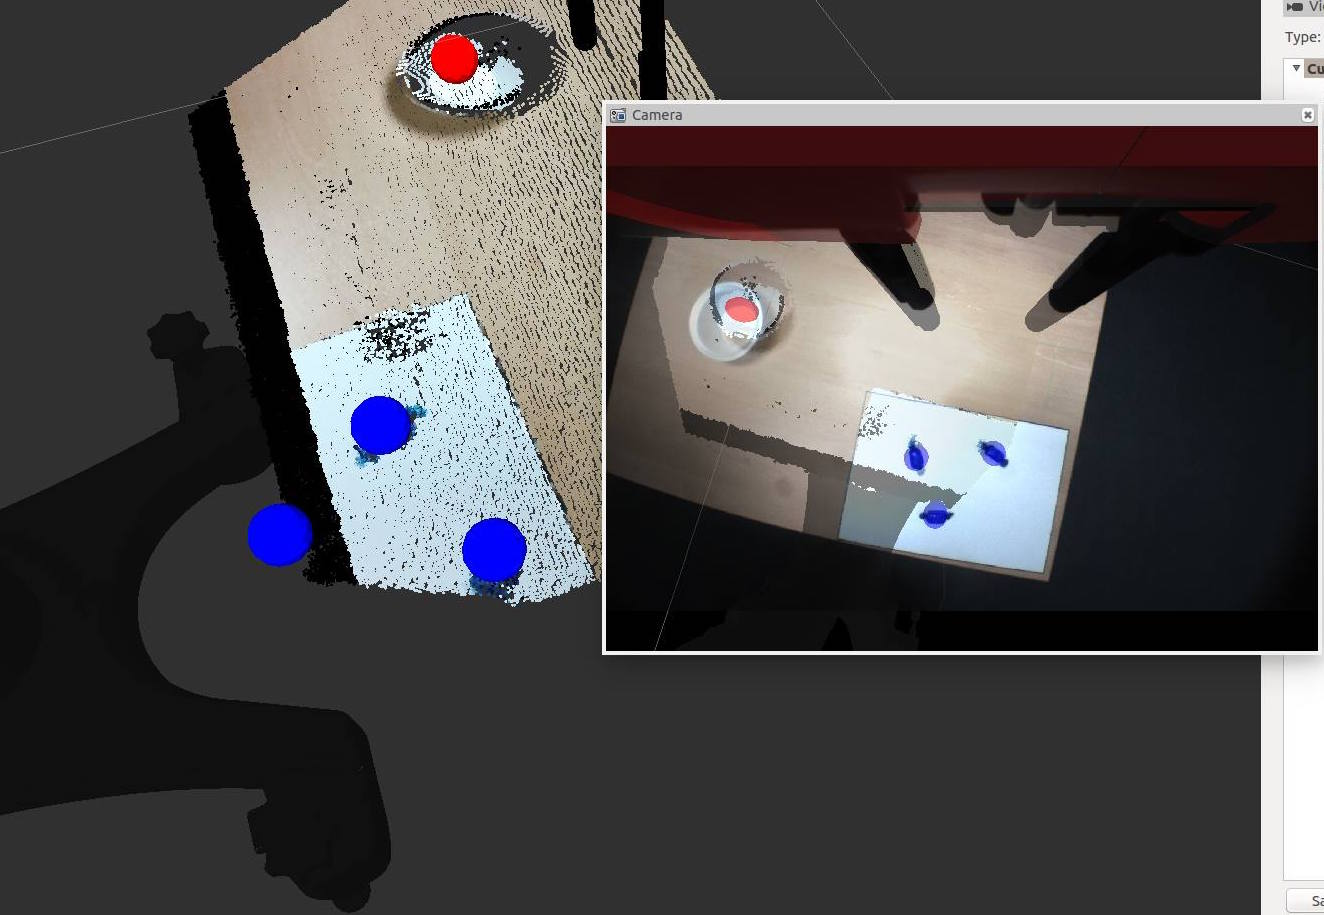
\includegraphics[width = 10cm, height = 6.5cm]{sweettransformation.jpg}
\centering
\captionof{figure}{\textit{An example of segmented objects}}
\bigskip
\end{minipage}
with dilation and erosion to close any incomplete edges, resulting in a reasonably successful edge detection for the entire image.
\newline
\newline
\begin{minipage}[t]{0.30\textwidth}
\raggedright
\smallskip
\textbf{Hough Line Transform}
\newline
Firstly, to find a rectangle in the image, Hough Line Transform was attempted to be used to find the individual edges of the paper. This technique was somewhat successful when attempting to distinguish between the edges however, by varying and optimising the line detection threshold, 
\smallskip
\end{minipage}
\hspace{0.5cm}
\begin{minipage}[t]{0.64\textwidth}
\smallskip
\centering
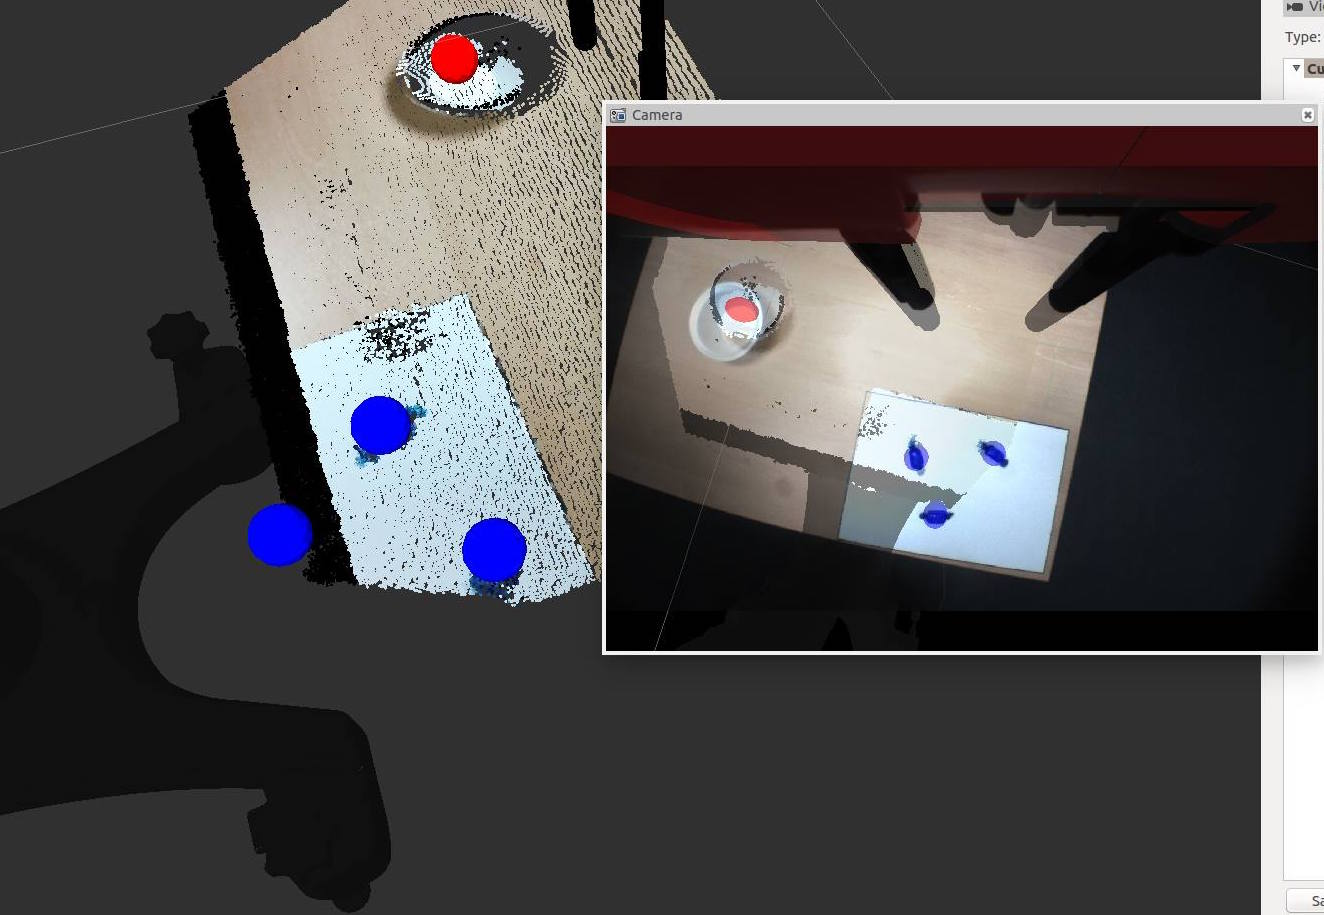
\includegraphics[width = 10cm, height = 6.5cm]{sweettransformation.jpg}
\centering
\captionof{figure}{\textit{An example of segmented objects}}
\bigskip
\end{minipage}
it was difficult to detect all four edges of the paper constantly. Either one or two edges kept being detected then undetected or too many edges were found. Due to the inaccuracy of this edge detection, the four edges could not always be found to form the rectangle. Therefore other methods were explored.
\newline
\newline
\textbf{Contour Detection}
\newline
\begin{minipage}[t]{0.64\textwidth}
\smallskip
\centering
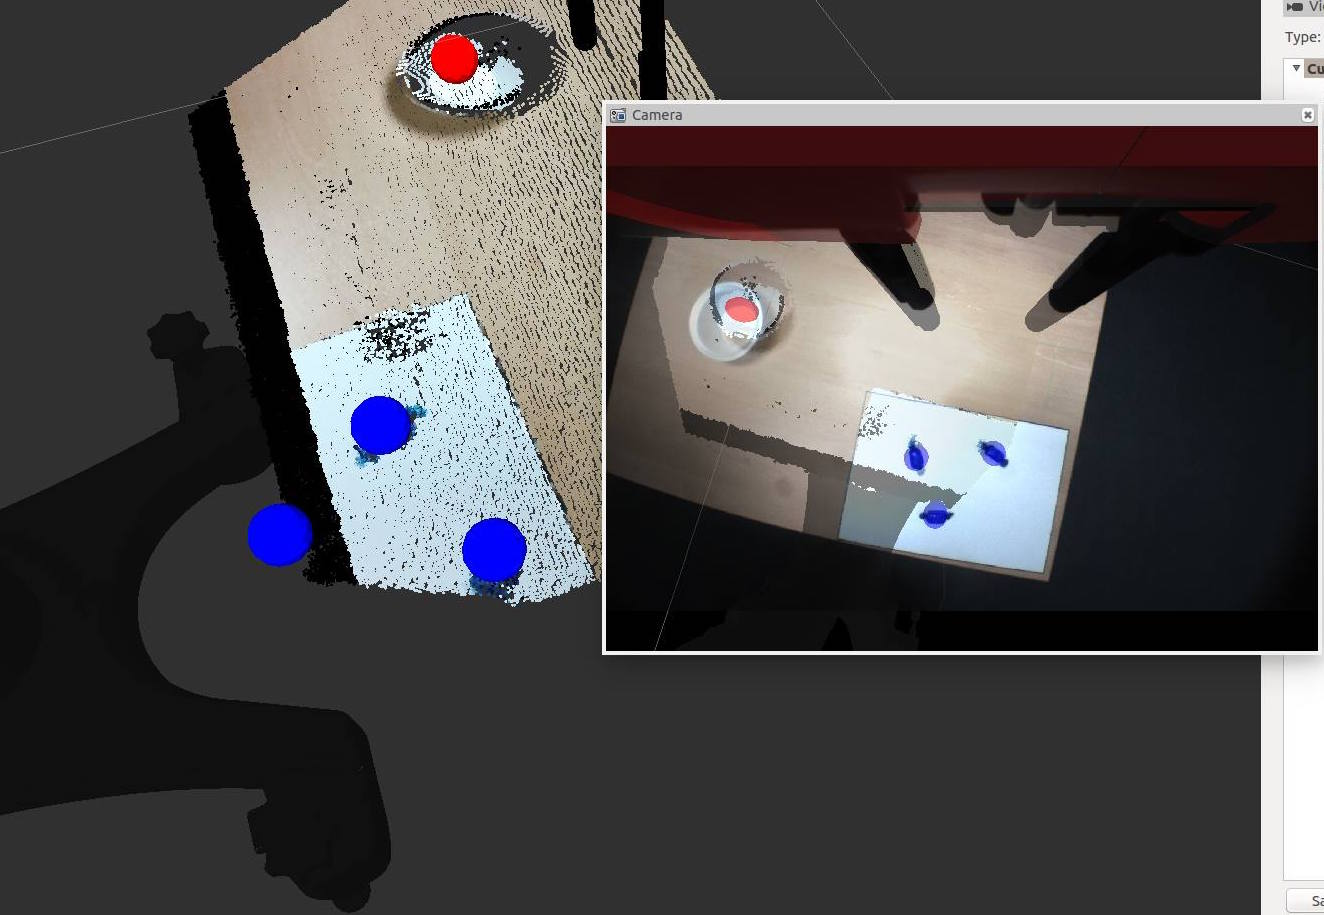
\includegraphics[width = 10cm, height = 6.5cm]{sweettransformation.jpg}
\centering
\captionof{figure}{\textit{An example of white colour segmented objects}}
\bigskip
\end{minipage}
\hspace{0.5cm}
\begin{minipage}[t]{0.29\textwidth}
\raggedright
Once the black border on the area was defined enough to be consistent during canny edge detection, a contour successfully managed to detect the four edges of the paper. Due to there being many contours detected in the image, certain constraints had to be put on the detection to segment out the sweet 
\end{minipage}	
area. The main method of segmenting out the rectangular area then was to first eliminate the smaller contours by size (using the in-built countourArea) and then approximate a polygon for the countours to detect which countour was a rectangle. This contour then produced a mask, which could segment out the rest of the image from the sweet area.
\newline
\newline
Once the sweet placement area was reliably segmented out from the image, multiple methods were used to attempt to try and identify the individual sweets. These methods are explained below:
\newline
\newline
\begin{minipage}[t]{0.30\textwidth}
\raggedright
\smallskip
\textbf{Hough Circle Transform}
\newline
For the simple, round sweets initially used in trials, a Hough Circle detection algorithm seemed like a sensible way to detect the simpler, round sweets. However, like the Hough Line detection used earlier, it was hard to get a constant solution, with circles  
\smallskip
\end{minipage}
\hspace{0.5cm}
\begin{minipage}[t]{0.64\textwidth}
\smallskip
\centering
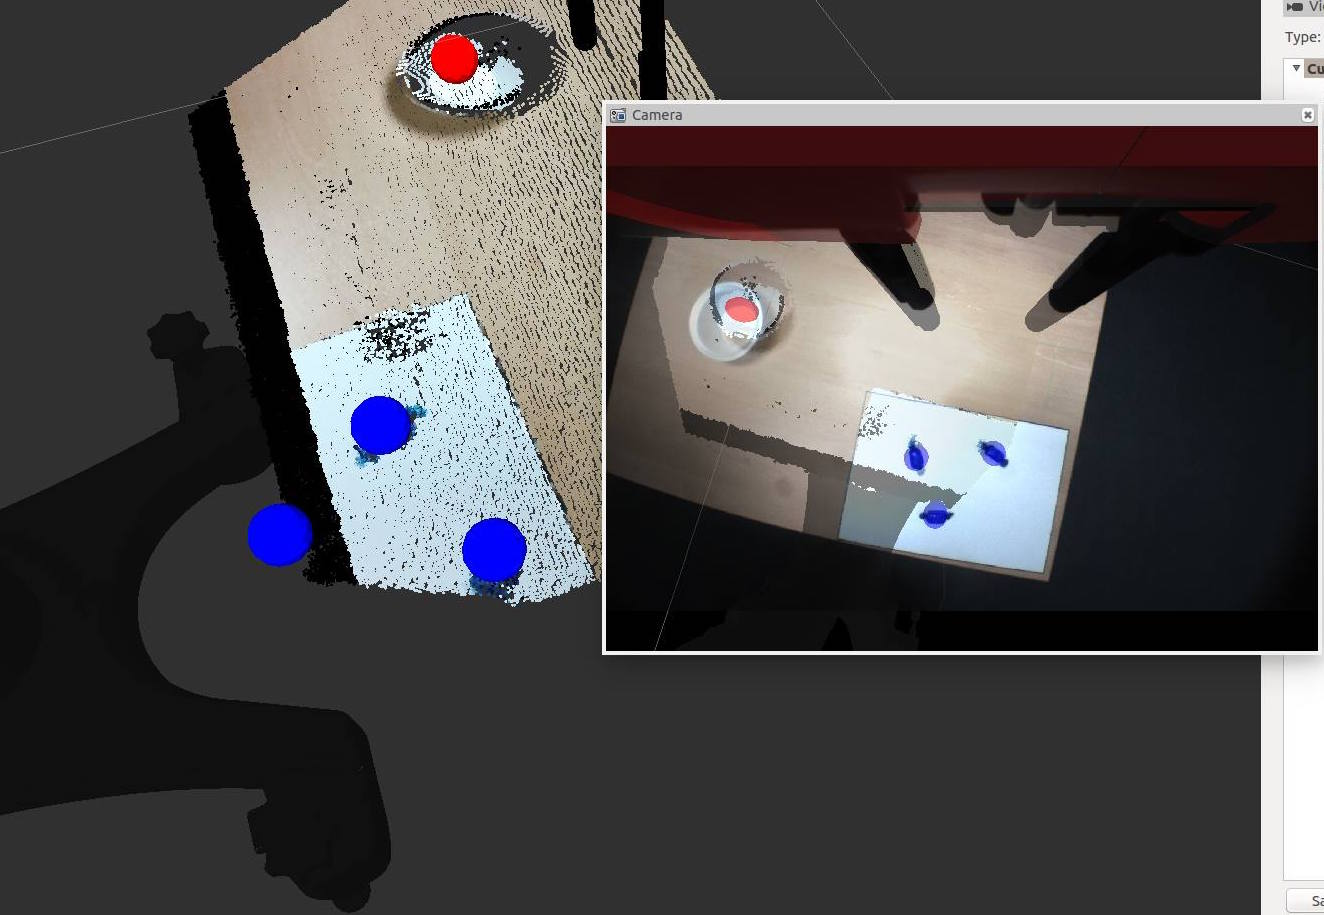
\includegraphics[width = 10cm, height = 6.5cm]{sweettransformation.jpg}
\centering
\captionof{figure}{\textit{An example of segmented objects}}
\bigskip
\end{minipage}
being detected and then undetected throughout various received image frames, therefore other methods needed to be tried to get a more reliable vision system.
\newline
\newline
\textbf{Contour Detection}
\newline
A better method was to do some image processing, Gaussian blurring, closing and opening to produce a lot better results, producing a mask of a white background with some black sweets in front. The problem with using this method is due to reflections on the sweets wrappers, this caused an issue of multiple broken contours within an individual sweet, whereas a preferred method would have been to capture the whole sweet with one contour, as Baxter needs to be able to count each sweet once.
\newline
\newline
\textbf{HSV Colour Segmentation with Contour Detection}
\newline
\begin{minipage}[t]{0.64\textwidth}
\smallskip
\centering
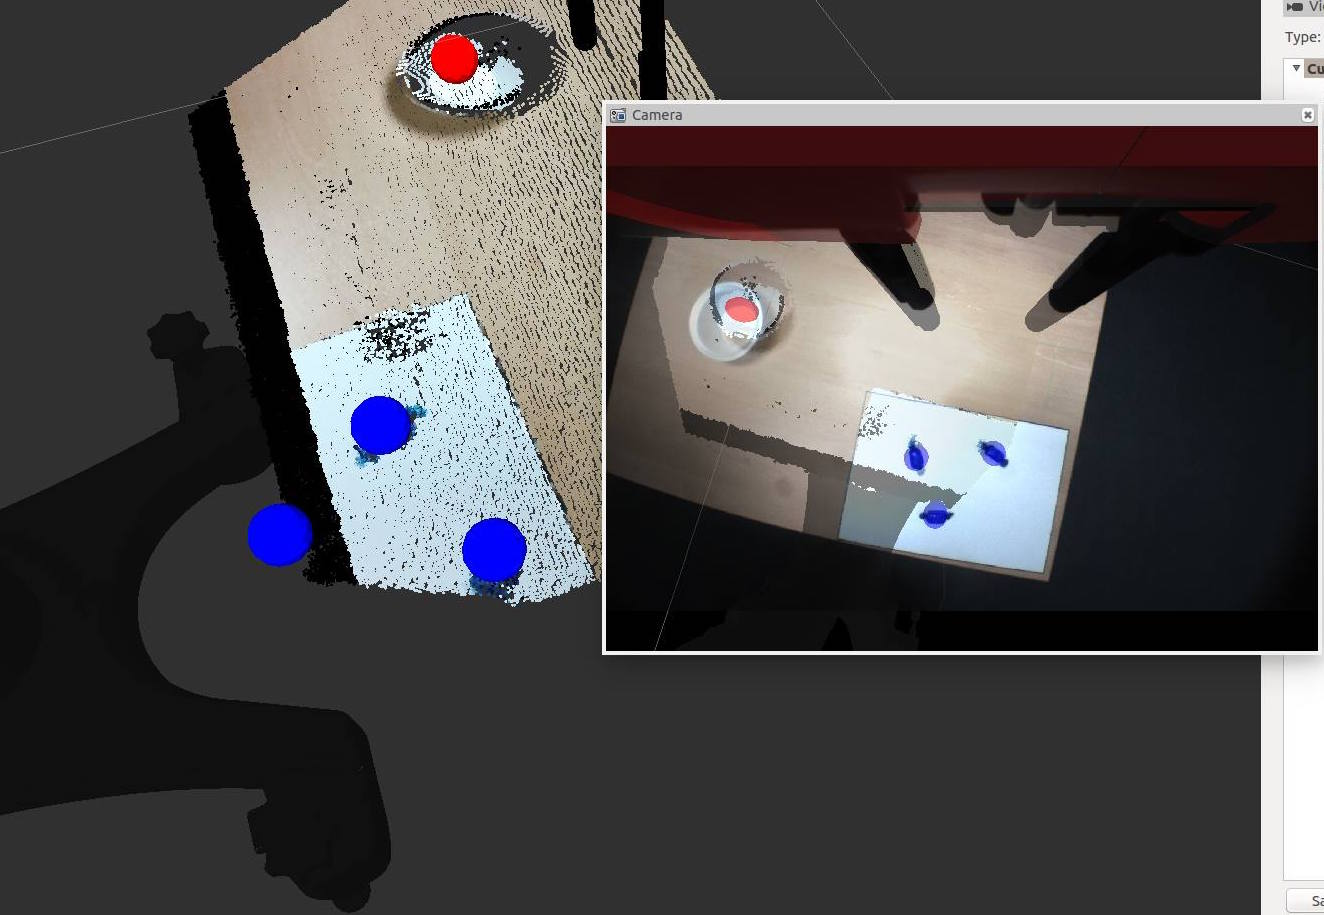
\includegraphics[width = 10cm, height = 6.5cm]{sweettransformation.jpg}
\centering
\captionof{figure}{\textit{An example of white colour segmented objects}}
\bigskip
\end{minipage}
\hspace{0.5cm}
\begin{minipage}[t]{0.29\textwidth}
\raggedright
A more accurate method was found by using an existing tool called objectfinder. This tool uses multiple sliders to segment an image and produce a mask using lower and upper bounds for RGB values. Since each sweet wrapper had different identifiable colours and they were placed onto a separatable 
\end{minipage}	
white background, using a scale of possible HSV values could be used to identify main sweet wrapper colours - blue, green, red etc. The only limitation of this approach was that similar colours under light could be mixed up, for example, red and pink wrappers had overlapping HSV RBG ranges, and therefore could not be both separated and identified by this method. It did however result in very clear contours for the significantly different colours so this method was used for the sweet recognition. Possible improvements could be made with shape recognition then colour analysis, which may have been able to identify a typical sweet shape and then separate by colour after.
\newline
\newline
Now there was a method for the sweets to be detected, by extracting moments from the sweet contours, the 2D pixel coordinate could be retrieved from the 2D image. The problem then was converting the 2D points in that image into 3D world coordinates. 
This was done using an altered version of a pinhole camera method, where the u, v coordinate within the 2D image could be converted to a 3D world coordinate using Baxter's in-built calibrated camera matrix. The equation uses the x and y camera offset values, with the focal lengths to scale the initial point. Then using the distance from the camera to the table (which is fixed), the points can then be converted into 3D world coordinates. This was tested using rViz and Baxter to make sure it worked.
\subsection{Sweet Singulation}
\section{The Manipulation System}
\subsection{Manipulating the Bowl}
\subsection{Sweet Manipulation}
\section{Human Interaction}
\subsection{Voice Recognition}
\subsection{Hand Recognition}
Pages to be referenced for practical applications:
\newline
\url{http://docs.opencv.org/3.0-beta/doc/py_tutorials/py_imgproc/py_houghlines/py_houghlines.html#py-hough-lines}
\url{http://docs.opencv.org/2.4/modules/calib3d/doc/camera_calibration_and_3d_reconstruction.html}
\url{http://pointclouds.org/documentation/tutorials/region_growing_segmentation.php}
\newline
\url{http://pointclouds.org/documentation/tutorials/region_growing_rgb_segmentation.php}
\newline
\url{http://wiki.ros.org/tabletop_object_detector}
\newline
\url{http://docs.pointclouds.org/trunk/group__sample__consensus.html}
\newline
\newline
~\cite{kinectfusion}
~\cite{objectlabelling}
~\cite{herbrobot}
~\cite{reliablegrasping}